% Options for packages loaded elsewhere
\PassOptionsToPackage{unicode}{hyperref}
\PassOptionsToPackage{hyphens}{url}
%
\documentclass[
]{article}
\usepackage{amsmath,amssymb}
\usepackage{lmodern}
\usepackage{ifxetex,ifluatex}
\ifnum 0\ifxetex 1\fi\ifluatex 1\fi=0 % if pdftex
  \usepackage[T1]{fontenc}
  \usepackage[utf8]{inputenc}
  \usepackage{textcomp} % provide euro and other symbols
\else % if luatex or xetex
  \usepackage{unicode-math}
  \defaultfontfeatures{Scale=MatchLowercase}
  \defaultfontfeatures[\rmfamily]{Ligatures=TeX,Scale=1}
\fi
% Use upquote if available, for straight quotes in verbatim environments
\IfFileExists{upquote.sty}{\usepackage{upquote}}{}
\IfFileExists{microtype.sty}{% use microtype if available
  \usepackage[]{microtype}
  \UseMicrotypeSet[protrusion]{basicmath} % disable protrusion for tt fonts
}{}
\makeatletter
\@ifundefined{KOMAClassName}{% if non-KOMA class
  \IfFileExists{parskip.sty}{%
    \usepackage{parskip}
  }{% else
    \setlength{\parindent}{0pt}
    \setlength{\parskip}{6pt plus 2pt minus 1pt}}
}{% if KOMA class
  \KOMAoptions{parskip=half}}
\makeatother
\usepackage{xcolor}
\IfFileExists{xurl.sty}{\usepackage{xurl}}{} % add URL line breaks if available
\IfFileExists{bookmark.sty}{\usepackage{bookmark}}{\usepackage{hyperref}}
\hypersetup{
  pdftitle={Classification using Naive Bayes},
  pdfauthor={Laura Sudupe Medinilla},
  hidelinks,
  pdfcreator={LaTeX via pandoc}}
\urlstyle{same} % disable monospaced font for URLs
\usepackage[margin=1in]{geometry}
\usepackage{color}
\usepackage{fancyvrb}
\newcommand{\VerbBar}{|}
\newcommand{\VERB}{\Verb[commandchars=\\\{\}]}
\DefineVerbatimEnvironment{Highlighting}{Verbatim}{commandchars=\\\{\}}
% Add ',fontsize=\small' for more characters per line
\usepackage{framed}
\definecolor{shadecolor}{RGB}{248,248,248}
\newenvironment{Shaded}{\begin{snugshade}}{\end{snugshade}}
\newcommand{\AlertTok}[1]{\textcolor[rgb]{0.94,0.16,0.16}{#1}}
\newcommand{\AnnotationTok}[1]{\textcolor[rgb]{0.56,0.35,0.01}{\textbf{\textit{#1}}}}
\newcommand{\AttributeTok}[1]{\textcolor[rgb]{0.77,0.63,0.00}{#1}}
\newcommand{\BaseNTok}[1]{\textcolor[rgb]{0.00,0.00,0.81}{#1}}
\newcommand{\BuiltInTok}[1]{#1}
\newcommand{\CharTok}[1]{\textcolor[rgb]{0.31,0.60,0.02}{#1}}
\newcommand{\CommentTok}[1]{\textcolor[rgb]{0.56,0.35,0.01}{\textit{#1}}}
\newcommand{\CommentVarTok}[1]{\textcolor[rgb]{0.56,0.35,0.01}{\textbf{\textit{#1}}}}
\newcommand{\ConstantTok}[1]{\textcolor[rgb]{0.00,0.00,0.00}{#1}}
\newcommand{\ControlFlowTok}[1]{\textcolor[rgb]{0.13,0.29,0.53}{\textbf{#1}}}
\newcommand{\DataTypeTok}[1]{\textcolor[rgb]{0.13,0.29,0.53}{#1}}
\newcommand{\DecValTok}[1]{\textcolor[rgb]{0.00,0.00,0.81}{#1}}
\newcommand{\DocumentationTok}[1]{\textcolor[rgb]{0.56,0.35,0.01}{\textbf{\textit{#1}}}}
\newcommand{\ErrorTok}[1]{\textcolor[rgb]{0.64,0.00,0.00}{\textbf{#1}}}
\newcommand{\ExtensionTok}[1]{#1}
\newcommand{\FloatTok}[1]{\textcolor[rgb]{0.00,0.00,0.81}{#1}}
\newcommand{\FunctionTok}[1]{\textcolor[rgb]{0.00,0.00,0.00}{#1}}
\newcommand{\ImportTok}[1]{#1}
\newcommand{\InformationTok}[1]{\textcolor[rgb]{0.56,0.35,0.01}{\textbf{\textit{#1}}}}
\newcommand{\KeywordTok}[1]{\textcolor[rgb]{0.13,0.29,0.53}{\textbf{#1}}}
\newcommand{\NormalTok}[1]{#1}
\newcommand{\OperatorTok}[1]{\textcolor[rgb]{0.81,0.36,0.00}{\textbf{#1}}}
\newcommand{\OtherTok}[1]{\textcolor[rgb]{0.56,0.35,0.01}{#1}}
\newcommand{\PreprocessorTok}[1]{\textcolor[rgb]{0.56,0.35,0.01}{\textit{#1}}}
\newcommand{\RegionMarkerTok}[1]{#1}
\newcommand{\SpecialCharTok}[1]{\textcolor[rgb]{0.00,0.00,0.00}{#1}}
\newcommand{\SpecialStringTok}[1]{\textcolor[rgb]{0.31,0.60,0.02}{#1}}
\newcommand{\StringTok}[1]{\textcolor[rgb]{0.31,0.60,0.02}{#1}}
\newcommand{\VariableTok}[1]{\textcolor[rgb]{0.00,0.00,0.00}{#1}}
\newcommand{\VerbatimStringTok}[1]{\textcolor[rgb]{0.31,0.60,0.02}{#1}}
\newcommand{\WarningTok}[1]{\textcolor[rgb]{0.56,0.35,0.01}{\textbf{\textit{#1}}}}
\usepackage{longtable,booktabs,array}
\usepackage{calc} % for calculating minipage widths
% Correct order of tables after \paragraph or \subparagraph
\usepackage{etoolbox}
\makeatletter
\patchcmd\longtable{\par}{\if@noskipsec\mbox{}\fi\par}{}{}
\makeatother
% Allow footnotes in longtable head/foot
\IfFileExists{footnotehyper.sty}{\usepackage{footnotehyper}}{\usepackage{footnote}}
\makesavenoteenv{longtable}
\usepackage{graphicx}
\makeatletter
\def\maxwidth{\ifdim\Gin@nat@width>\linewidth\linewidth\else\Gin@nat@width\fi}
\def\maxheight{\ifdim\Gin@nat@height>\textheight\textheight\else\Gin@nat@height\fi}
\makeatother
% Scale images if necessary, so that they will not overflow the page
% margins by default, and it is still possible to overwrite the defaults
% using explicit options in \includegraphics[width, height, ...]{}
\setkeys{Gin}{width=\maxwidth,height=\maxheight,keepaspectratio}
% Set default figure placement to htbp
\makeatletter
\def\fps@figure{htbp}
\makeatother
\setlength{\emergencystretch}{3em} % prevent overfull lines
\providecommand{\tightlist}{%
  \setlength{\itemsep}{0pt}\setlength{\parskip}{0pt}}
\setcounter{secnumdepth}{-\maxdimen} % remove section numbering
\usepackage[spanish]{babel}
\ifluatex
  \usepackage{selnolig}  % disable illegal ligatures
\fi

\title{Classification using Naive Bayes}
\usepackage{etoolbox}
\makeatletter
\providecommand{\subtitle}[1]{% add subtitle to \maketitle
  \apptocmd{\@title}{\par {\large #1 \par}}{}{}
}
\makeatother
\subtitle{Predict flowering type depending plant genotype}
\author{Laura Sudupe Medinilla}
\date{12 de abril, 2021}

\begin{document}
\maketitle

{
\setcounter{tocdepth}{2}
\tableofcontents
}
\pagebreak

\hypertarget{naive-bayes-algorithm}{%
\section{Naive Bayes Algorithm}\label{naive-bayes-algorithm}}

The \emph{Naive Byes} algorithm describes a simple method to aplly Bayes
theorem to classification problems. Althopugh it is not the only machine
learning method that utilizes Bayesian methods, it is the most common
one. This is particularly true for text classification, where it has
become the de facto standard. The strengths and weaknesses of this
algorithm are as follows:

\begin{longtable}[]{@{}
  >{\raggedright\arraybackslash}p{(\columnwidth - 2\tabcolsep) * \real{0.40}}
  >{\raggedright\arraybackslash}p{(\columnwidth - 2\tabcolsep) * \real{0.60}}@{}}
\toprule
\textbf{Strenghts} & \textbf{Weaknesses} \\
\midrule
\endhead
* Simple, fast, and very effective & * SRelies on an often-faulty
assumption of equally important and independent features \\
* Does well with noisy and missing data & * Not ideal for datasets with
many numeric features \\
* Requires relatively few examples for training, but also works well
with very large numbers of examples & * Estimated probabilities are less
reliable than the predicted classes \\
* Easy to obtain the estimated probability for a prediction & \\
\bottomrule
\end{longtable}

\hypertarget{step-1---collecting-the-data}{%
\section{Step 1 - Collecting the
data}\label{step-1---collecting-the-data}}

This algorithm objetive is to predict the flowering type (fast or slow)
in function of the flower genotype.

We know the genotype of 697 flowers and the flowering day. We have 149
genotypes as predictor features. The genotype states are 0, 1 or 2,
which belong to dominant homozygote, heterozygote and recessive
homozigote.

\hypertarget{step-2---exploring-and-preparing-the-data}{%
\section{Step 2 - Exploring and preparing the
data}\label{step-2---exploring-and-preparing-the-data}}

The first step towards constructing our classifier involves processing
the raw data for analysis.

Using the \texttt{str()} function, we see our data structure

\begin{verbatim}
'data.frame':   697 obs. of  149 variables:
 $ gtype.1  : num  0 0 2 2 2 0 2 0 0 0 ...
 $ gtype.2  : num  2 1 2 0 2 0 0 0 2 2 ...
 $ gtype.3  : num  2 2 2 0 0 0 0 2 2 0 ...
 $ gtype.4  : num  2 2 0 0 0 0 2 0 2 2 ...
 $ gtype.5  : num  0 0 0 0 0 0 0 0 0 2 ...
  [list output truncated]
\end{verbatim}

The element are numeric, it would be better to convert it into a factor

Check again the structure

\begin{verbatim}
'data.frame':   697 obs. of  149 variables:
 $ gtype.1  : Factor w/ 3 levels "0","1","2": 1 1 3 3 3 1 3 1 1 1 ...
 $ gtype.2  : Factor w/ 3 levels "0","1","2": 3 2 3 1 3 1 1 1 3 3 ...
 $ gtype.3  : Factor w/ 3 levels "0","1","2": 3 3 3 1 1 1 1 3 3 1 ...
 $ gtype.4  : Factor w/ 3 levels "0","1","2": 3 3 1 1 1 1 3 1 3 3 ...
 $ gtype.5  : Factor w/ 2 levels "0","2": 1 1 1 1 1 1 1 1 1 2 ...
  [list output truncated]
\end{verbatim}

We need to create a new feature, \emph{fast} or \emph{slow} flowering.
If the number of days is higher or same to 40 days, we codifice like 1,
else, 0.

Take a look to the plants type numbers

\begin{verbatim}
flowering_factor
fast slow 
 437  260 
\end{verbatim}

\hypertarget{creating-training-and-test-datasets}{%
\subsection{- Creating training and test
datasets}\label{creating-training-and-test-datasets}}

We now need to split the data into training and test datasets.

\begin{Shaded}
\begin{Highlighting}[]
\FunctionTok{set.seed}\NormalTok{(params}\SpecialCharTok{$}\NormalTok{valor.seed)}
\NormalTok{train }\OtherTok{\textless{}{-}} \FunctionTok{sample}\NormalTok{(}\FunctionTok{nrow}\NormalTok{(genotype\_f),}\FunctionTok{floor}\NormalTok{(}\FunctionTok{nrow}\NormalTok{(genotype\_f)}\SpecialCharTok{*}\NormalTok{params}\SpecialCharTok{$}\NormalTok{p))}
\FunctionTok{length}\NormalTok{(train)}
\end{Highlighting}
\end{Shaded}

\begin{verbatim}
[1] 464
\end{verbatim}

\begin{Shaded}
\begin{Highlighting}[]
\NormalTok{train\_data }\OtherTok{\textless{}{-}}\NormalTok{ genotype\_f[train,]}
\NormalTok{test\_data }\OtherTok{\textless{}{-}}\NormalTok{ genotype\_f[}\SpecialCharTok{{-}}\NormalTok{train,]}

\NormalTok{class\_train }\OtherTok{\textless{}{-}}\NormalTok{ flowering\_factor[train]}
\NormalTok{class\_test }\OtherTok{\textless{}{-}}\NormalTok{ flowering\_factor[}\SpecialCharTok{{-}}\NormalTok{train]}
\end{Highlighting}
\end{Shaded}

\hypertarget{step-3---training-a-model-on-the-data}{%
\section{Step 3 - Training a model on the
data}\label{step-3---training-a-model-on-the-data}}

The Naive Bayes implementation we will employ in the e1071 package.
Build the classifier

\begin{Shaded}
\begin{Highlighting}[]
\FunctionTok{library}\NormalTok{(e1071)}
\NormalTok{m }\OtherTok{\textless{}{-}} \FunctionTok{naiveBayes}\NormalTok{(train\_data, class\_train, }\AttributeTok{laplace=}\DecValTok{0}\NormalTok{)}
\end{Highlighting}
\end{Shaded}

The function will return a naive Bayes model object that can be used to
make predictions

\hypertarget{step-4---evaluatin-model-performance}{%
\section{Step 4 - Evaluatin model
performance}\label{step-4---evaluatin-model-performance}}

To evaluate the flowering classifier, we need to test its predictions on
unseen test data. The \texttt{predict()} function is used to make the
predictions

The function will return a vector of predicted class values ç

\begin{Shaded}
\begin{Highlighting}[]
\NormalTok{test\_pred }\OtherTok{\textless{}{-}} \FunctionTok{predict}\NormalTok{(m, test\_data)}
\end{Highlighting}
\end{Shaded}

To compare the predictions to the true values, we´ll use the
\texttt{CrossTable()} function

\begin{Shaded}
\begin{Highlighting}[]
\FunctionTok{library}\NormalTok{(gmodels)}
\FunctionTok{CrossTable}\NormalTok{(}\AttributeTok{x =}\NormalTok{test\_pred , }\AttributeTok{y =}\NormalTok{ class\_test , }\AttributeTok{prop.chisq=}\ConstantTok{FALSE}\NormalTok{)}
\end{Highlighting}
\end{Shaded}

\begin{verbatim}
 
   Cell Contents
|-------------------------|
|                       N |
|           N / Row Total |
|           N / Col Total |
|         N / Table Total |
|-------------------------|

 
Total Observations in Table:  233 

 
             | class_test 
   test_pred |      fast |      slow | Row Total | 
-------------|-----------|-----------|-----------|
        fast |       116 |        43 |       159 | 
             |     0.730 |     0.270 |     0.682 | 
             |     0.817 |     0.473 |           | 
             |     0.498 |     0.185 |           | 
-------------|-----------|-----------|-----------|
        slow |        26 |        48 |        74 | 
             |     0.351 |     0.649 |     0.318 | 
             |     0.183 |     0.527 |           | 
             |     0.112 |     0.206 |           | 
-------------|-----------|-----------|-----------|
Column Total |       142 |        91 |       233 | 
             |     0.609 |     0.391 |           | 
-------------|-----------|-----------|-----------|

 
\end{verbatim}

\hypertarget{step-5---improving-model-performance}{%
\section{Step 5 - Improving model
performance}\label{step-5---improving-model-performance}}

We are going to do the same but we will set a value for the Laplace
estimator

\begin{Shaded}
\begin{Highlighting}[]
\NormalTok{m2 }\OtherTok{\textless{}{-}} \FunctionTok{naiveBayes}\NormalTok{(train\_data, class\_train, }\AttributeTok{laplace=}\DecValTok{1}\NormalTok{)}
\end{Highlighting}
\end{Shaded}

Do the prediction

\begin{Shaded}
\begin{Highlighting}[]
\NormalTok{test\_pred2 }\OtherTok{\textless{}{-}} \FunctionTok{predict}\NormalTok{(m2, test\_data)}
\end{Highlighting}
\end{Shaded}

Evaluate the model

\begin{Shaded}
\begin{Highlighting}[]
\CommentTok{\#library(gmodels)}
\FunctionTok{CrossTable}\NormalTok{(}\AttributeTok{x =}\NormalTok{test\_pred2 , }\AttributeTok{y =}\NormalTok{ class\_test , }\AttributeTok{prop.chisq=}\ConstantTok{FALSE}\NormalTok{)}
\end{Highlighting}
\end{Shaded}

\begin{verbatim}
 
   Cell Contents
|-------------------------|
|                       N |
|           N / Row Total |
|           N / Col Total |
|         N / Table Total |
|-------------------------|

 
Total Observations in Table:  233 

 
             | class_test 
  test_pred2 |      fast |      slow | Row Total | 
-------------|-----------|-----------|-----------|
        fast |       116 |        42 |       158 | 
             |     0.734 |     0.266 |     0.678 | 
             |     0.817 |     0.462 |           | 
             |     0.498 |     0.180 |           | 
-------------|-----------|-----------|-----------|
        slow |        26 |        49 |        75 | 
             |     0.347 |     0.653 |     0.322 | 
             |     0.183 |     0.538 |           | 
             |     0.112 |     0.210 |           | 
-------------|-----------|-----------|-----------|
Column Total |       142 |        91 |       233 | 
             |     0.609 |     0.391 |           | 
-------------|-----------|-----------|-----------|

 
\end{verbatim}

The results are very similar between them

\hypertarget{roc-curve}{%
\section{ROC curve}\label{roc-curve}}

We will performe the ROC value for each case \texttt{laplace=0} y
\texttt{laplace=\ 1}.

\hypertarget{case-laplace0}{%
\subsection{\texorpdfstring{Case
\texttt{laplace=0}}{Case laplace=0}}\label{case-laplace0}}

First of all we will obtain the flowering probabilities for each plant
in the test data

\begin{Shaded}
\begin{Highlighting}[]
\NormalTok{test\_pred\_roc }\OtherTok{\textless{}{-}} \FunctionTok{predict}\NormalTok{(m, test\_data, }\AttributeTok{type=}\StringTok{"raw"}\NormalTok{)}
\end{Highlighting}
\end{Shaded}

With the positive class probabilities, we performe the ROC curve

\begin{Shaded}
\begin{Highlighting}[]
\NormalTok{pred\_roc }\OtherTok{\textless{}{-}} \FunctionTok{prediction}\NormalTok{(}\AttributeTok{predictions=}\NormalTok{ test\_pred\_roc[,}\DecValTok{2}\NormalTok{], }\AttributeTok{labels=}\NormalTok{class\_test)}
\NormalTok{perf\_roc }\OtherTok{\textless{}{-}} \FunctionTok{performance}\NormalTok{(pred\_roc, }\AttributeTok{measure=}\StringTok{"tpr"}\NormalTok{, }\AttributeTok{x.measure=}\StringTok{"fpr"}\NormalTok{)}
\CommentTok{\#unlist(perf\_roc@alpha.values)}


\FunctionTok{plot}\NormalTok{(perf\_roc, }\AttributeTok{main=} \StringTok{"ROC curve"}\NormalTok{, }\AttributeTok{col=} \StringTok{"blue"}\NormalTok{, }\AttributeTok{lwd=}\DecValTok{3}\NormalTok{, }\AttributeTok{colorize=}\ConstantTok{TRUE}\NormalTok{)}
\FunctionTok{abline}\NormalTok{(}\AttributeTok{a=}\DecValTok{0}\NormalTok{, }\AttributeTok{b=} \DecValTok{1}\NormalTok{, }\AttributeTok{lwd=} \DecValTok{2}\NormalTok{, }\AttributeTok{lty =} \DecValTok{2}\NormalTok{)}
\end{Highlighting}
\end{Shaded}

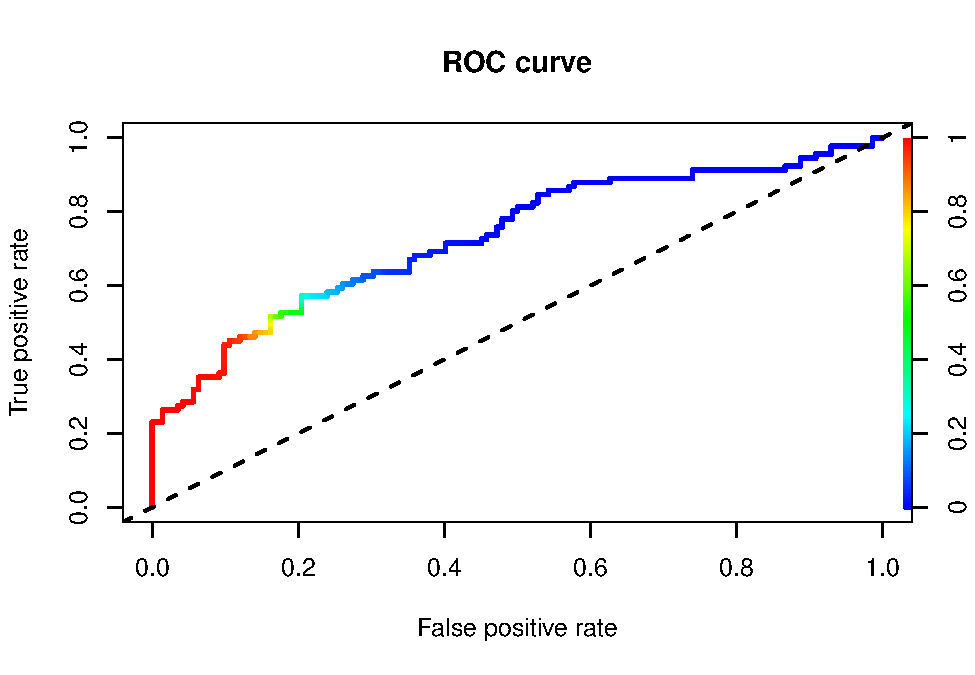
\includegraphics{naive_bayes_laura_files/figure-latex/unnamed-chunk-16-1.pdf}

\begin{Shaded}
\begin{Highlighting}[]
\NormalTok{perf.auc }\OtherTok{\textless{}{-}} \FunctionTok{performance}\NormalTok{(pred\_roc, }\AttributeTok{measure =}\StringTok{"auc"}\NormalTok{)}
\end{Highlighting}
\end{Shaded}

AUC value is \textbf{0.7303823}.

\hypertarget{case-laplace1}{%
\subsection{\texorpdfstring{Case
\texttt{laplace=1}}{Case laplace=1}}\label{case-laplace1}}

First of all we will obtain the flowering probabilities for each plant
in the test data

\begin{Shaded}
\begin{Highlighting}[]
\NormalTok{test\_pred2 }\OtherTok{\textless{}{-}} \FunctionTok{predict}\NormalTok{(m2, test\_data, }\AttributeTok{type=}\StringTok{"raw"}\NormalTok{)}
\end{Highlighting}
\end{Shaded}

With the positive class probabilities, we performe the ROC curve

\begin{Shaded}
\begin{Highlighting}[]
\NormalTok{pred2 }\OtherTok{\textless{}{-}} \FunctionTok{prediction}\NormalTok{(}\AttributeTok{predictions=}\NormalTok{ test\_pred2[,}\DecValTok{2}\NormalTok{], }\AttributeTok{labels=}\NormalTok{class\_test)}
\NormalTok{perf2 }\OtherTok{\textless{}{-}} \FunctionTok{performance}\NormalTok{(pred2, }\AttributeTok{measure=}\StringTok{"tpr"}\NormalTok{, }\AttributeTok{x.measure=}\StringTok{"fpr"}\NormalTok{)}
\CommentTok{\#unlist(perf@alpha.values)}


\FunctionTok{plot}\NormalTok{(perf2, }\AttributeTok{main=} \StringTok{"ROC curve"}\NormalTok{, }\AttributeTok{col=} \StringTok{"blue"}\NormalTok{, }\AttributeTok{lwd=}\DecValTok{3}\NormalTok{, }\AttributeTok{colorize=}\ConstantTok{TRUE}\NormalTok{)}
\FunctionTok{abline}\NormalTok{(}\AttributeTok{a=}\DecValTok{0}\NormalTok{, }\AttributeTok{b=} \DecValTok{1}\NormalTok{, }\AttributeTok{lwd=} \DecValTok{2}\NormalTok{, }\AttributeTok{lty =} \DecValTok{2}\NormalTok{)}
\end{Highlighting}
\end{Shaded}

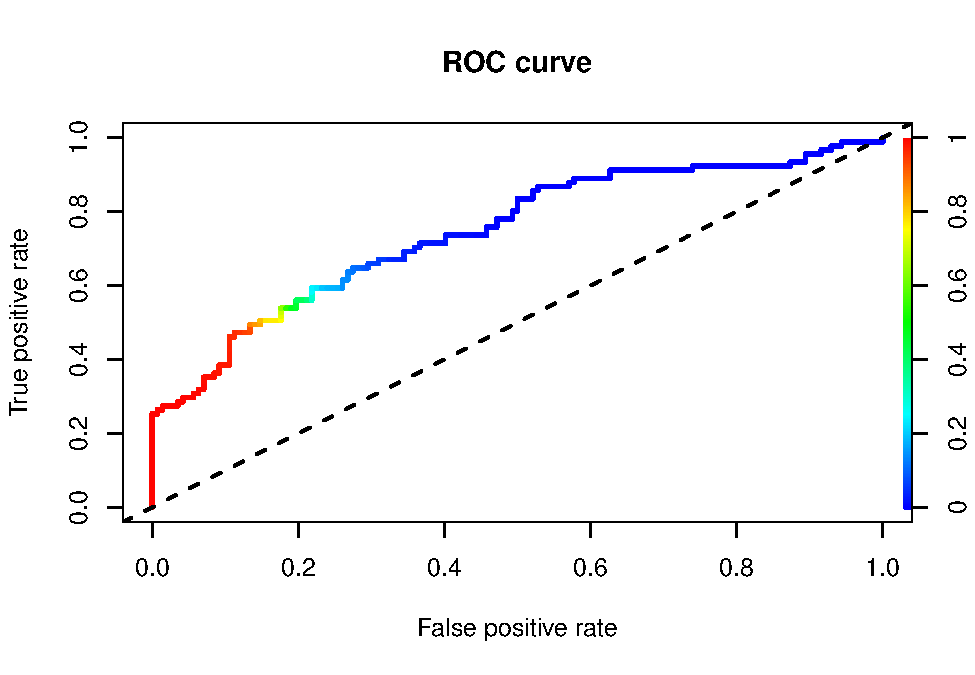
\includegraphics{naive_bayes_laura_files/figure-latex/unnamed-chunk-18-1.pdf}

\begin{Shaded}
\begin{Highlighting}[]
\NormalTok{perf2.auc }\OtherTok{\textless{}{-}} \FunctionTok{performance}\NormalTok{(pred2, }\AttributeTok{measure =}\StringTok{"auc"}\NormalTok{)}


\CommentTok{\#str(perf)}
\end{Highlighting}
\end{Shaded}

AUC value is \textbf{0.7450085}.

\end{document}
